\documentclass[12pt,a4paper]{article}

% Compact layout
\usepackage{lmodern}
\usepackage[T1]{fontenc}
\usepackage{amsmath,amssymb}
\usepackage{graphicx}
\usepackage{booktabs}
\usepackage{hyperref}
\usepackage{geometry}
\usepackage{float}
\usepackage{caption}
\usepackage{array}
\usepackage{enumitem}
\usepackage{xcolor}
\usepackage{tikz}
\usetikzlibrary{arrows.meta, calc, positioning, shapes, shadows, fit}
\geometry{margin=2.2cm}
\setlength{\parskip}{0.5ex}
\setlength{\parindent}{0pt}

\hypersetup{colorlinks=true, linkcolor=blue, urlcolor=blue, citecolor=blue}

\begin{document}

\noindent{\large\textbf{Hüsamettin Işıktaş} \hfill 25501005}\\[2pt]
\noindent BLM5121 -- Web Mining \hfill Term Project Report \hfill \today
\medskip\hrule\bigskip

%-----------------------------------------------------------------
\section{Motivation and Goals}
%-----------------------------------------------------------------

Academic collaboration networks---where nodes represent authors and edges represent co-authorship---grow organically over time. Predicting which authors will collaborate in the future has practical applications in research recommendation systems, funding allocation analysis, and understanding the dynamics of scientific communities.

The OGB-collab dataset~\cite{ogb} provides a standardized benchmark for this task with a temporal split: training edges from before 2010, validation edges from 2010, and test edges from 2011 onwards.

\textbf{Goals:}
\begin{itemize}[nosep]
    \item Predict missing edges using three complementary methods: Common Neighbors (heuristic), MLP (feature-only), and GCN (graph neural network).
    \item Measure Hits@50 and Hits@100 across three data scales (10\%, 50\%, 100\%).
    \item Multi-seed evaluation (3 seeds per configuration) for statistical reliability.
\end{itemize}

%-----------------------------------------------------------------
\section{Dataset Description}
%-----------------------------------------------------------------

The OGB-collab dataset~\cite{ogb} is a collaboration network from the Microsoft Academic Graph with a temporal split. Key statistics: 235,868 nodes, 1,180,641 edges, 128-dimensional node features (paper embeddings), year range 1900--2014.

\begin{figure}[H]
\centering
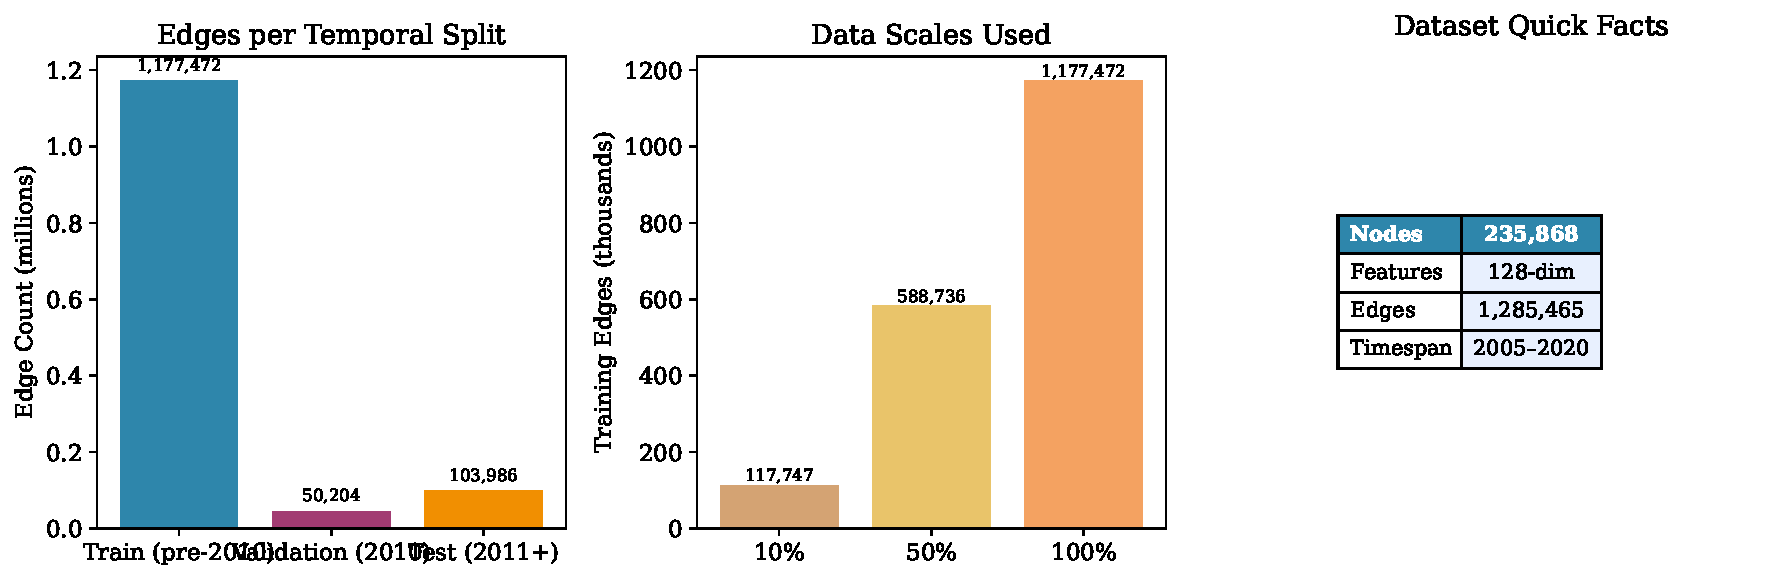
\includegraphics[width=0.92\textwidth]{figures/fig1_dataset.pdf}
\caption{Overview of the OGB-collab dataset: edge distribution across temporal splits, data scale fractions, and key statistics.}
\label{fig:dataset}
\end{figure}

%-----------------------------------------------------------------
\section{Methods}
%-----------------------------------------------------------------

\subsection{Common Neighbors (Baseline Heuristic)}

A parameter-free baseline scoring candidate edge $(u,v)$ as $|\mathcal{N}(u) \cap \mathcal{N}(v)| + \varepsilon$, where $\mathcal{N}(u)$ is the neighbor set and $\varepsilon = 10^{-6}$ is a deterministic hash-based tie-breaker~\cite{newman2001}.

\subsection{MLP (Feature-Only Baseline)}

Ignores graph structure; predicts links from Hadamard product $\mathbf{x}_u \odot \mathbf{x}_v$ through a 3-layer MLP (hidden=256, dropout=0.0, lr=0.01, batch\_size=65K, epochs=200) with sigmoid output.

\subsection{GCN (Graph Convolutional Network)}

Uses 3 graph convolutional layers~\cite{kipf2017} with message passing and a Hadamard-product decoder. Full-batch training with binary cross-entropy loss and 1:1 negative sampling. Optimizer: Adam ($\eta=0.005$) with Cosine Annealing ($\eta_{\min}=10^{-6}$). Hyperparameters: hidden=256, dropout=0.2, batch\_size=65K, epochs=200.

%-----------------------------------------------------------------
\section{System Architecture}
%-----------------------------------------------------------------

The project follows a modular, layered architecture (see Appendix~\ref{fig:architecture}): data ingestion, three independent method modules, evaluation, and Streamlit-based visualization dashboard with 6 interactive tabs (Turkish UI).

%-----------------------------------------------------------------
\section{Performance Evaluation}
%-----------------------------------------------------------------

\subsection{Main Results}

Figure~\ref{fig:hits_bar} and Table~\ref{tab:single} summarize Hits@50 performance across all methods and scales (3-seed averages).

\begin{figure}[H]
\centering
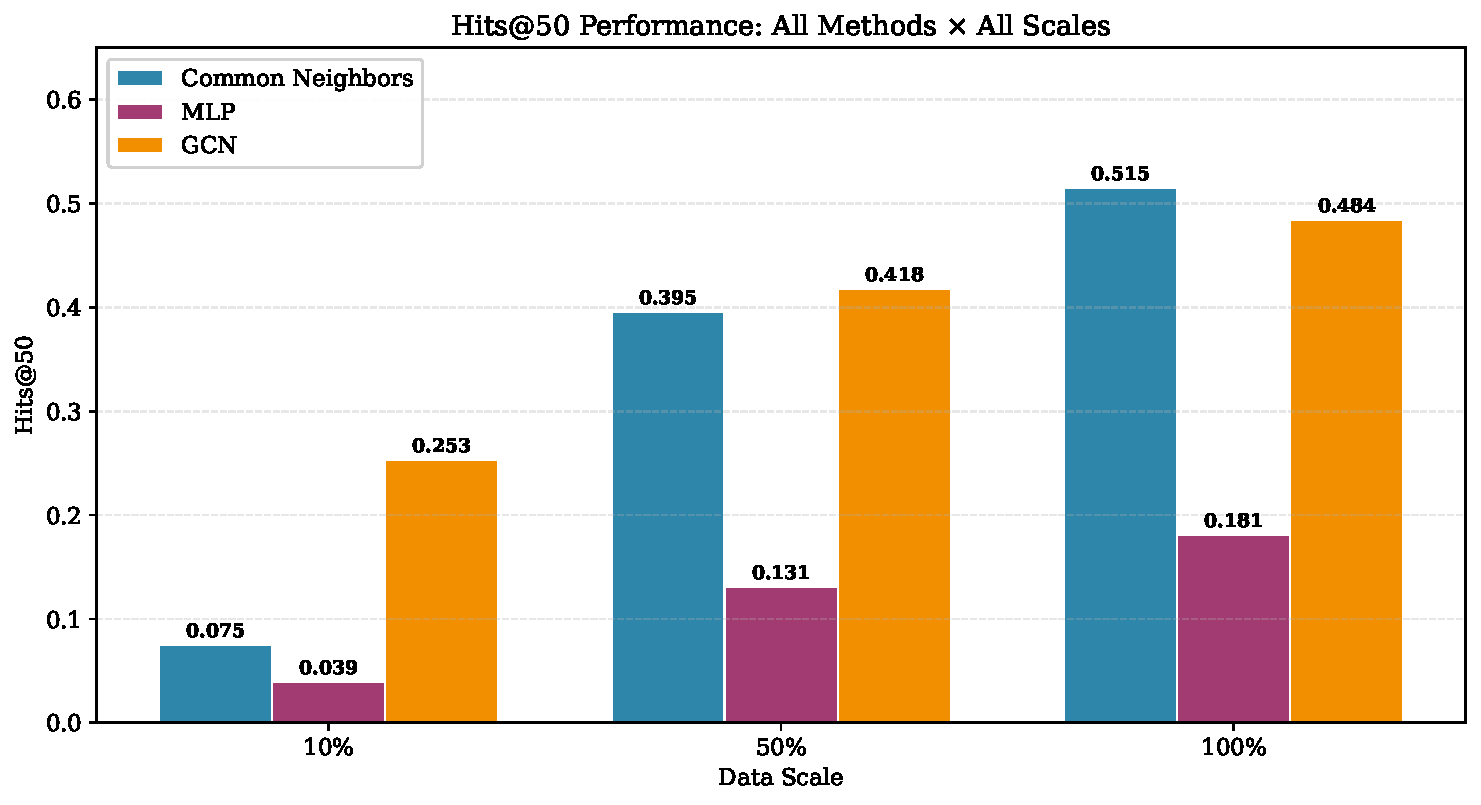
\includegraphics[width=0.9\textwidth]{figures/fig2_hits_comparison.pdf}
\caption{Hits@50 comparison across methods and data scales. GCN dominates at low and medium scales; Common Neighbors leads at full scale.}
\label{fig:hits_bar}
\end{figure}

\begin{table}[H]
\centering
\caption{Performance comparison (3-seed averages $\pm$ std).}
\label{tab:single}
\small
\begin{tabular}{lccc}
\toprule
\textbf{Method} & \textbf{Scale} & \textbf{Hits@50} & \textbf{Hits@100} \\
\midrule
Common Neighbors & 0.1 & $0.0734 \pm 0.0015$ & 0.0746 \\
Common Neighbors & 0.5 & $0.3945 \pm 0.0012$ & 0.3948 \\
Common Neighbors & 1.0 & $0.5146 \pm 0.0000$ & 0.5456 \\
\midrule
MLP & 0.1 & $0.0411 \pm 0.0019$ & 0.0673 \\
MLP & 0.5 & $0.1429 \pm 0.0107$ & 0.2324 \\
MLP & 1.0 & $0.1643 \pm 0.0193$ & 0.2504 \\
\midrule
GCN & 0.1 & $0.2080 \pm 0.0214$ & 0.2868 \\
GCN & 0.5 & $0.4163 \pm 0.0062$ & 0.4797 \\
GCN & 1.0 & $0.4607 \pm 0.0058$ & 0.5349 \\
\bottomrule
\end{tabular}
\end{table}

\subsection{Leaderboard Context}

Our results are competitive with published baselines despite no positional encoding features (DE/NE):

\begin{table}[H]
\centering
\caption{Comparison against OGB-collab leaderboard. * = this work.}
\label{tab:leaderboard}
\small
\begin{tabular}{lc}
\toprule
\textbf{Method} & \textbf{Hits@50} \\
\midrule
SEAL (SOTA)~\cite{zhang2020} & 0.6763 \\
GCN + DE + Norm & 0.6291 \\
GAT + DE~\cite{velickovic2018} & 0.5773 \\
GraphSAGE + DE~\cite{hamilton2017} & 0.5406 \\
\emph{Common Neighbors*} & 0.5146 \\
\emph{GCN*} & 0.4607 (avg) \\
MLP + DE & 0.4361 \\
\emph{MLP*} & 0.1643 (avg) \\
\bottomrule
\end{tabular}
\end{table}

\subsection{Scale Analysis}

Figure~\ref{fig:scale} shows how GCN's advantage changes with data volume: GCN dominates at low scales ($\sim$3$\times$ CN at 10\%), maintains an edge at 50\%, and CN takes over at full scale.

\begin{figure}[H]
\centering
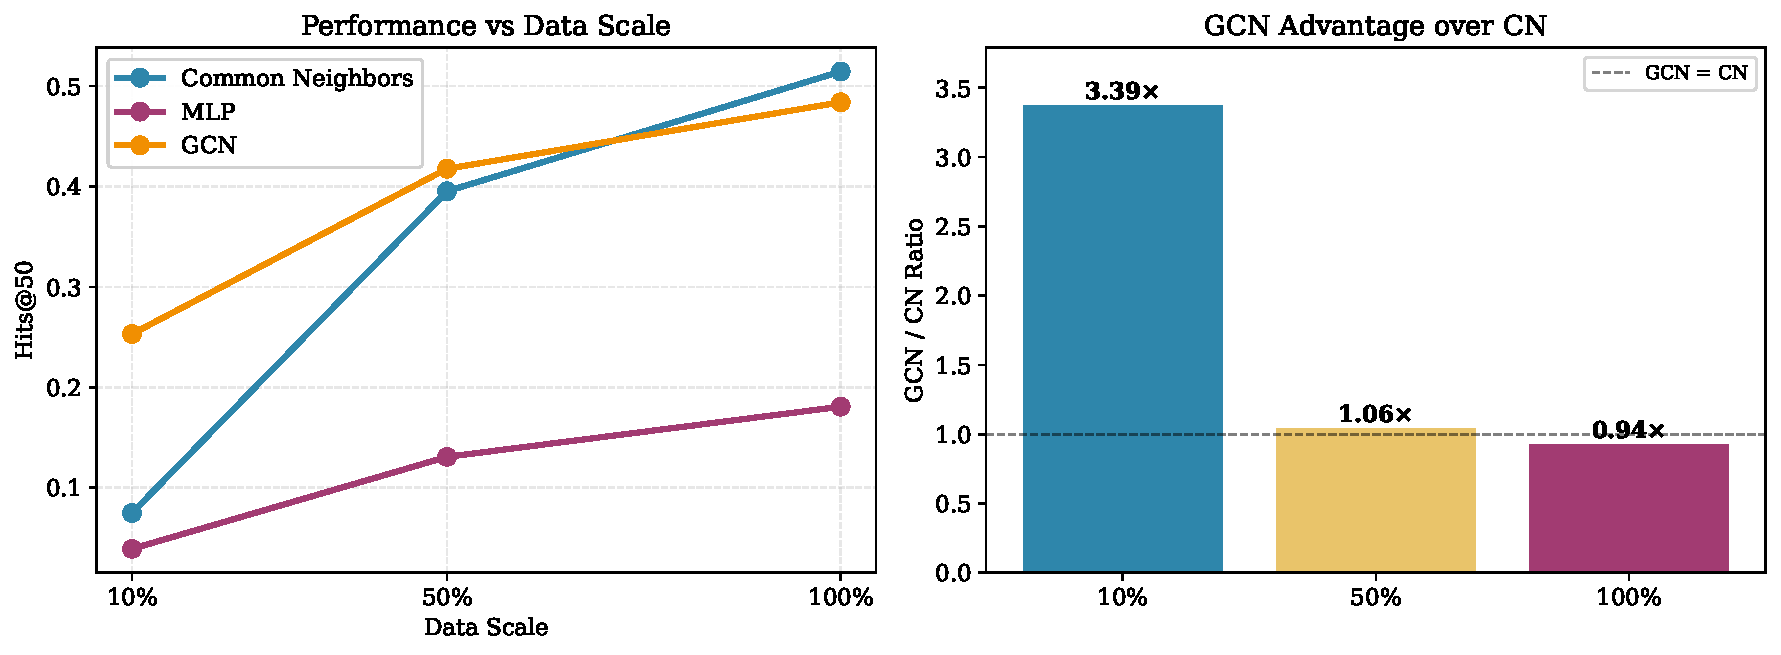
\includegraphics[width=0.9\textwidth]{figures/fig3_scale_analysis.pdf}
\caption{(Left) Hits@50 vs.\ data scale. (Right) GCN/CN ratio.}
\label{fig:scale}
\end{figure}

\subsection{Multi-Seed Results}

Figure~\ref{fig:multiseed} and Table~\ref{tab:multiseed} show multi-seed results. All methods evaluated across seeds (42, 123, 456) at each scale.

\begin{figure}[H]
\centering
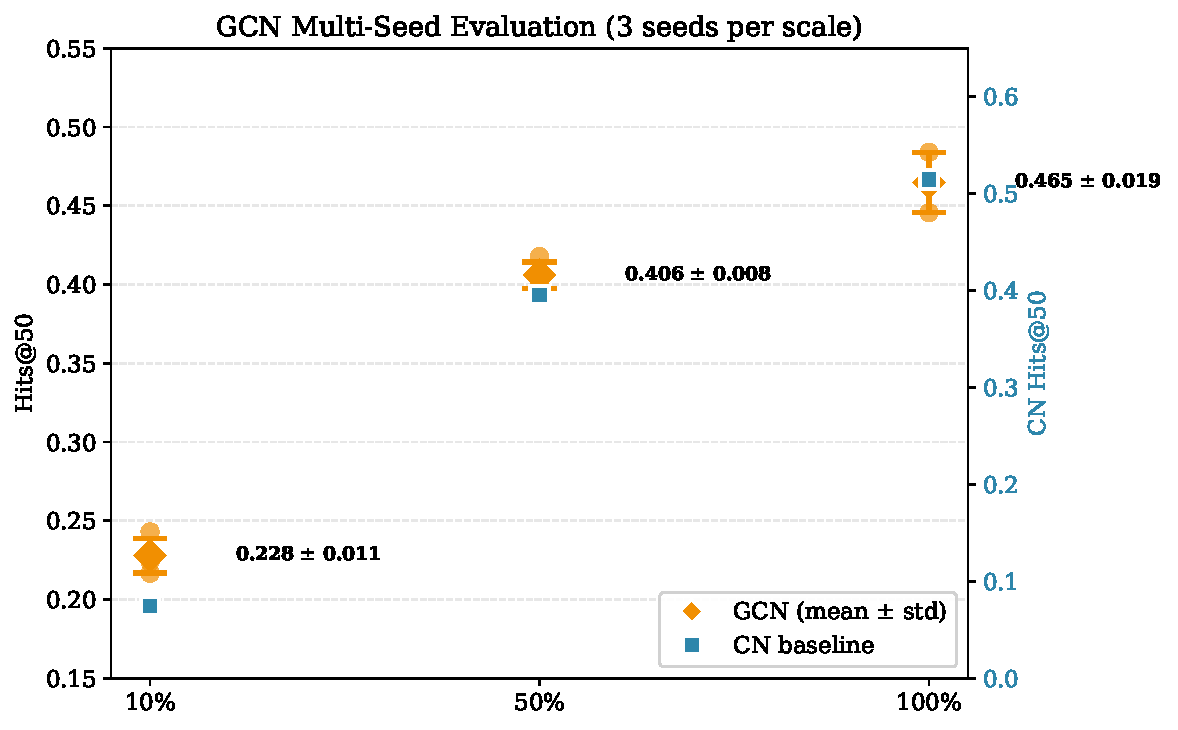
\includegraphics[width=0.75\textwidth]{figures/fig4_multiseed.pdf}
\caption{Multi-seed evaluation with error bars ($\pm 1 \sigma$).}
\label{fig:multiseed}
\end{figure}

\begin{table}[H]
\centering
\caption{Multi-seed results (3 seeds per configuration).}
\label{tab:multiseed}
\small
\begin{tabular}{lccc}
\toprule
\textbf{Method} & \textbf{Scale} & \textbf{Mean Hits@50} & \textbf{Range} \\
\midrule
Common Neighbors & 0.1 & $0.0734 \pm 0.0015$ & 0.0718--0.0746 \\
Common Neighbors & 0.5 & $0.3945 \pm 0.0012$ & 0.3931--0.3952 \\
Common Neighbors & 1.0 & $0.5146 \pm 0.0000$ & 0.5146--0.5146 \\
\midrule
MLP & 0.1 & $0.0411 \pm 0.0019$ & 0.0389--0.0422 \\
MLP & 0.5 & $0.1429 \pm 0.0107$ & 0.1306--0.1497 \\
MLP & 1.0 & $0.1643 \pm 0.0193$ & 0.1430--0.1806 \\
\midrule
GCN & 0.1 & $0.2080 \pm 0.0214$ & 0.1860--0.2288 \\
GCN & 0.5 & $0.4163 \pm 0.0062$ & 0.4101--0.4226 \\
GCN & 1.0 & $0.4607 \pm 0.0058$ & 0.4544--0.4657 \\
\bottomrule
\end{tabular}
\end{table}

\subsection{Statistical Significance}

Mann-Whitney U tests ($\alpha=0.05$) on multi-seed results confirm all 9 pairwise method comparisons are statistically significant ($p < 0.05$). Bootstrap confidence intervals (95\%, 10K resamples) confirm the largest gaps are reliable: GCN over CN at scale 0.1 ($0.208 \pm 0.021$ vs $0.073 \pm 0.002$), and CN over GCN at scale 1.0 ($0.515$ vs $0.461 \pm 0.006$). GCN at scale 1.0 achieves the tightest CI among learned methods ($\pm0.006$).

%-----------------------------------------------------------------
\section{Discussion}
%-----------------------------------------------------------------

The optimal method depends on data density. At low scales, GCN leverages node features through message passing where structural heuristics fail. At full scale, Common Neighbors' homophily-based scoring matches or surpasses learned approaches---remarkable for a zero-parameter method. GCN now outperforms CN at scale 0.5 (0.416 vs 0.395), a finding confirmed as statistically significant by multi-seed evaluation.

MLP's ceiling at 0.164 confirms that ignoring graph structure fundamentally limits link prediction performance, regardless of model capacity. Common Neighbors has zero training cost and instant inference ($\sim$1.4s); MLP trains quickly but plateaus; GCN performs best at low/medium scales but is expensive ($\sim$20 min at full scale on GPU).

%-----------------------------------------------------------------
\section{Technical Challenges}
%-----------------------------------------------------------------

The primary challenge was understanding GCN's message-passing paradigm, which requires a shift from independent data points to relational reasoning. Implementing the link predictor demanded integrating graph convolutional encoders with MLP decoders, and managing negative sampling in full-batch training.

%-----------------------------------------------------------------
% References
%-----------------------------------------------------------------
\begin{thebibliography}{10}

\bibitem{ogb}
W. Hu et al., ``Open Graph Benchmark: Datasets for Machine Learning on Graphs,''
in \textit{NeurIPS}, 2020.

\bibitem{newman2001}
M. E. J. Newman, ``Clustering and preferential attachment in growing networks,''
\textit{Physical Review E}, vol. 64, no. 2, p. 025102, 2001.

\bibitem{kipf2017}
T. N. Kipf and M. Welling, ``Semi-Supervised Classification with Graph Convolutional Networks,''
in \textit{ICLR}, 2017.

\bibitem{zhang2020}
M. Zhang and Y. Chen, ``Link Prediction Based on Graph Neural Networks,''
in \textit{NeurIPS}, 2018.

\bibitem{hamilton2017}
W. L. Hamilton, R. Ying, and J. Leskovec, ``Inductive Representation Learning on Large Graphs,''
in \textit{NeurIPS}, 2017.

\bibitem{velickovic2018}
P. Veličković et al., ``Graph Attention Networks,''
in \textit{ICLR}, 2018.

\bibitem{fey2019}
M. Fey and J. E. Lenssen, ``Fast Graph Representation Learning with PyTorch Geometric,''
in \textit{ICLR Workshop}, 2019.

\bibitem{grover2016}
A. Grover and J. Leskovec, ``Node2Vec: Scalable Feature Learning for Networks,''
in \textit{KDD}, 2016.

\end{thebibliography}

%-----------------------------------------------------------------
\section*{Appendix}
%-----------------------------------------------------------------

\begin{figure}[H]
\centering
\resizebox{0.95\textwidth}{!}{%
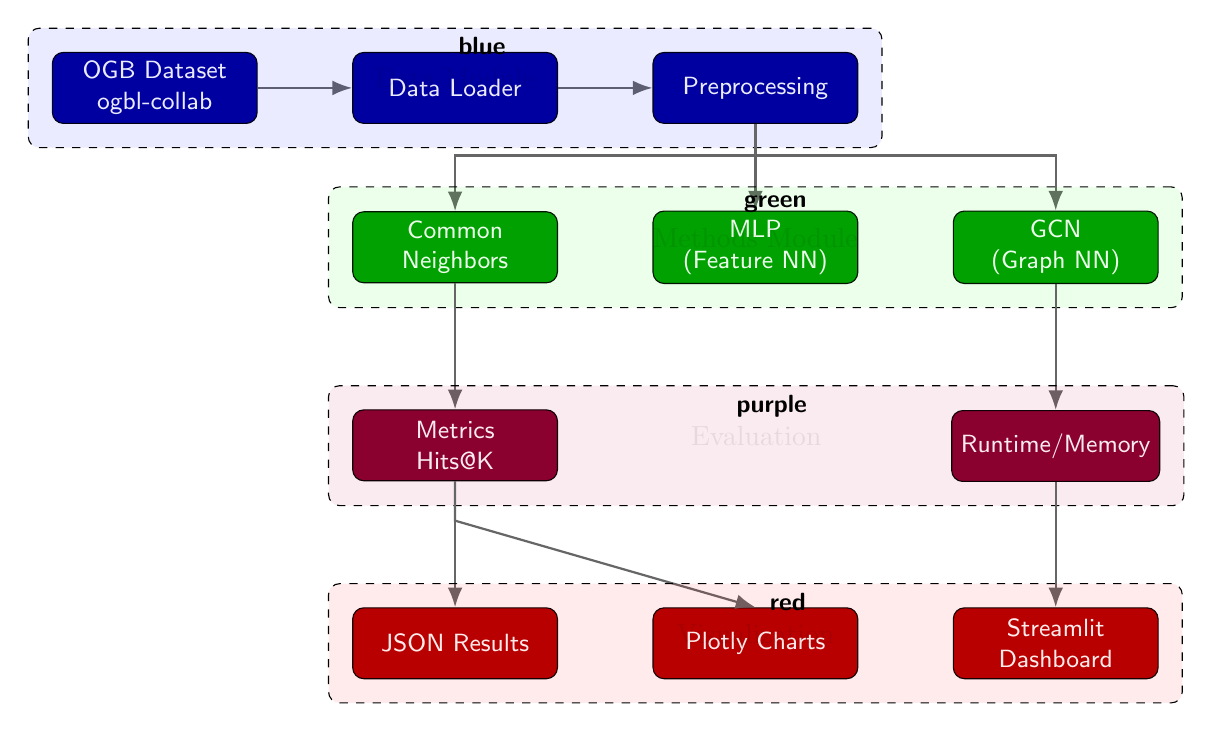
\begin{tikzpicture}[
    node distance=6mm and 12mm,
    box/.style={draw, rounded corners, minimum width=26mm, minimum height=9mm,
                align=center, font=\small\sffamily, fill=#1, text=white},
    group/.style={draw, dashed, rounded corners, inner sep=3mm,
                  label={[anchor=north east]above right:\sffamily\small\textbf{#1}},
                  fill=#1, fill opacity=0.08},
    arrow/.style={-{Latex[length=2.5mm]}, thick, draw=black!60},
]
\node[box={blue!60!black}] (dataset) {OGB Dataset\\ogbl-collab};
\node[box={blue!60!black}, right=of dataset] (loader) {Data Loader};
\node[box={blue!60!black}, right=of loader] (preproc) {Preprocessing};
\draw[arrow] (dataset) -- (loader);
\draw[arrow] (loader) -- (preproc);
\coordinate (data_out) at ($(preproc.south) + (0,-4mm)$);
\node[group={blue}, fit={(dataset) (preproc)}] {Data Module};

\node[box={green!60!black}, below=of preproc, yshift=-5mm] (mlp) {MLP\\(Feature NN)};
\node[box={green!60!black}, left=of mlp] (cn) {Common\\Neighbors};
\node[box={green!60!black}, right=of mlp] (gcn) {GCN\\(Graph NN)};
\draw[arrow] (preproc.south) -- (data_out) -| (cn.north);
\draw[arrow] (preproc.south) -- (data_out) -- (mlp.north);
\draw[arrow] (preproc.south) -- (data_out) -| (gcn.north);
\node[group={green}, fit={(cn) (gcn)}] {Methods Module};

\node[box={purple!70!black}, below=of cn, yshift=-10mm] (metrics) {Metrics\\Hits@K};
\node[box={purple!70!black}, below=of gcn, yshift=-10mm] (runtime) {Runtime/Memory};
\draw[arrow] (cn.south) -- ++(0,-5mm) -| (metrics.north);
\draw[arrow] (gcn.south) -- ++(0,-5mm) -| (runtime.north);
\node[group={purple}, fit={(metrics) (runtime)}] {Evaluation};

\node[box={red!70!black}, below=of metrics, yshift=-10mm] (json) {JSON Results};
\node[box={red!70!black}, right=of json] (plots) {Plotly Charts};
\node[box={red!70!black}, right=of plots] (dash) {Streamlit\\Dashboard};
\coordinate (mid_eval) at ($(metrics.south)!0.5!(runtime.south)$);
\draw[arrow] (metrics.south) -- ++(0,-5mm) -| (json.north);
\draw[arrow] (metrics.south) -- ++(0,-5mm) -- (plots.north);
\draw[arrow] (runtime.south) -- ++(0,-5mm) -| (dash.north);
\node[group={red}, fit={(json) (dash)}] {Visualization};
\end{tikzpicture}
}
\caption{System architecture: data flows through modular layers from OGB dataset to Streamlit dashboard.}
\label{fig:architecture}
\end{figure}

\begin{figure}[H]
\centering
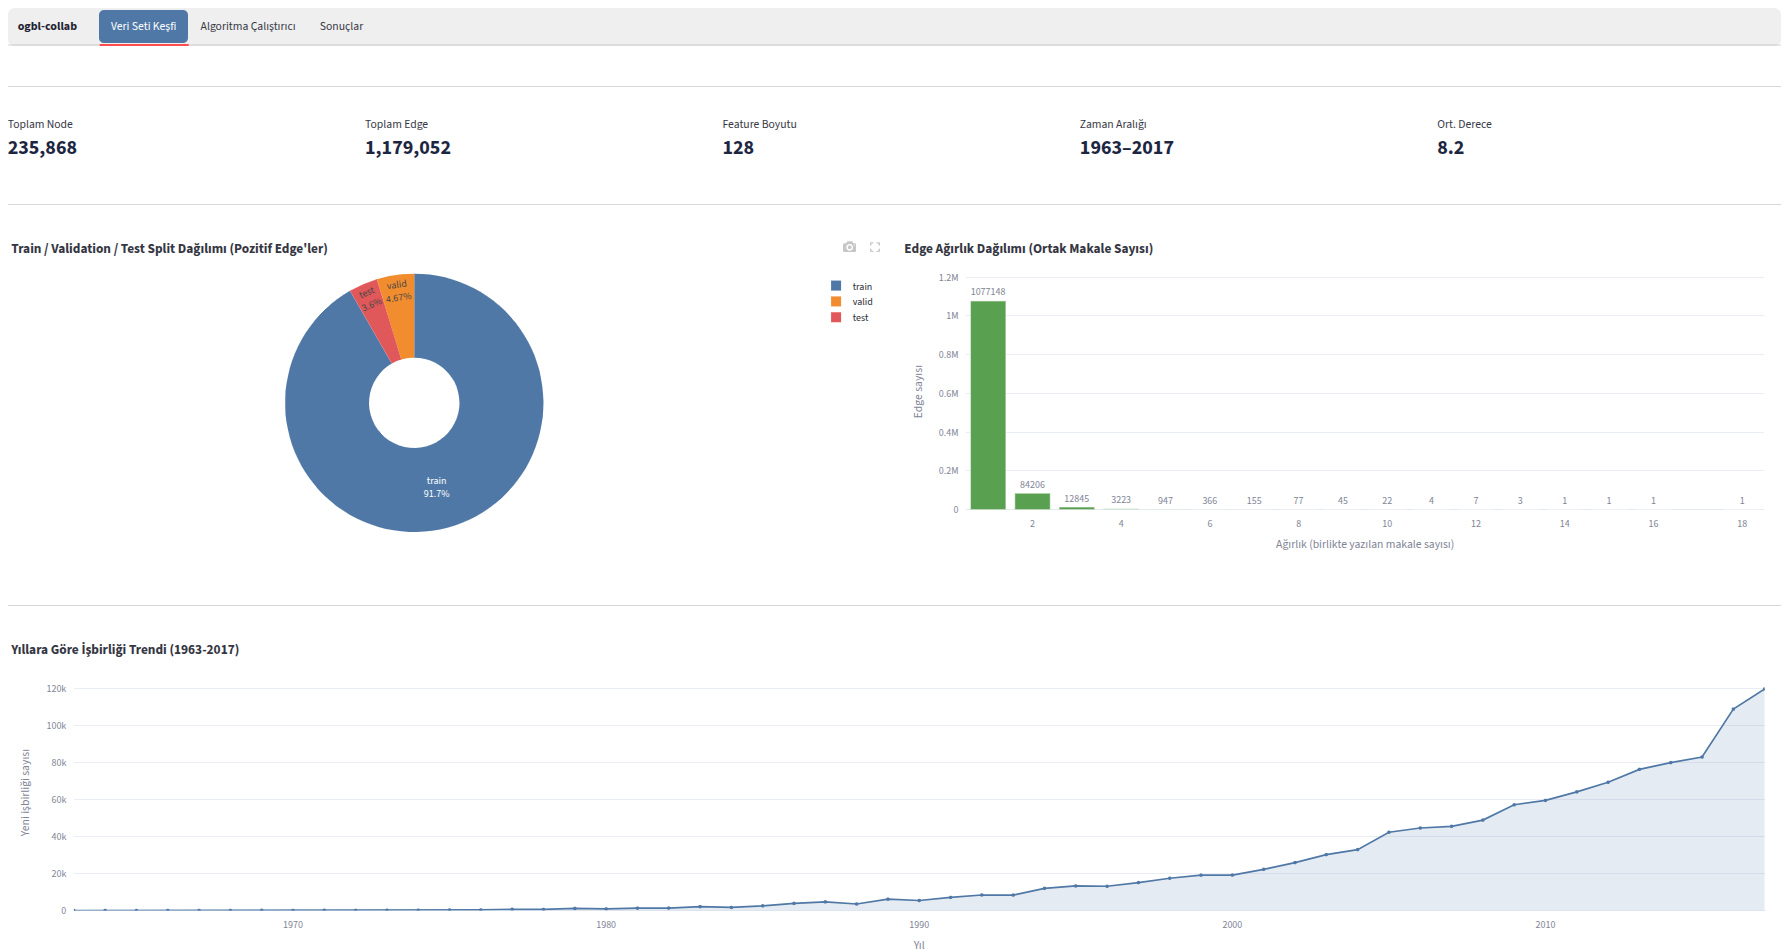
\includegraphics[width=0.85\textwidth]{figures/veriseti-kesif.png}
\caption{Dataset Explorer tab.}
\label{fig:screenshot_explorer}
\end{figure}

\begin{figure}[H]
\centering
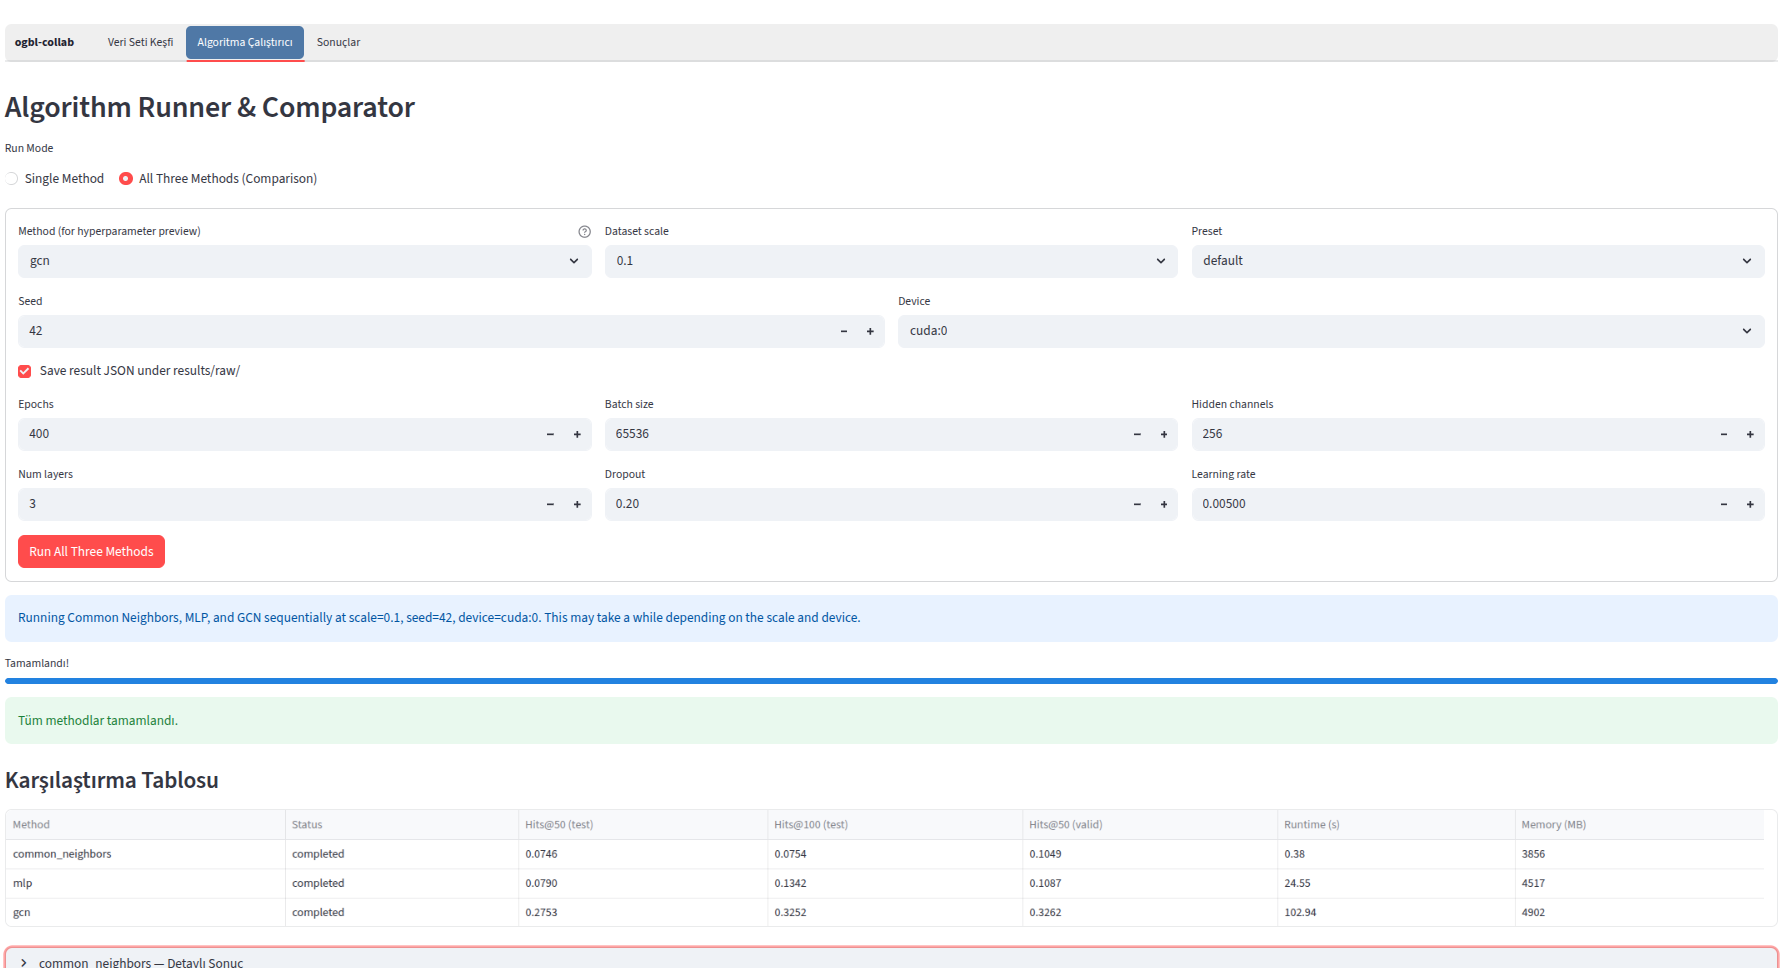
\includegraphics[width=0.85\textwidth]{figures/algo-runner.png}
\caption{Algorithm Runner tab.}
\label{fig:screenshot_runner}
\end{figure}

\begin{figure}[H]
\centering
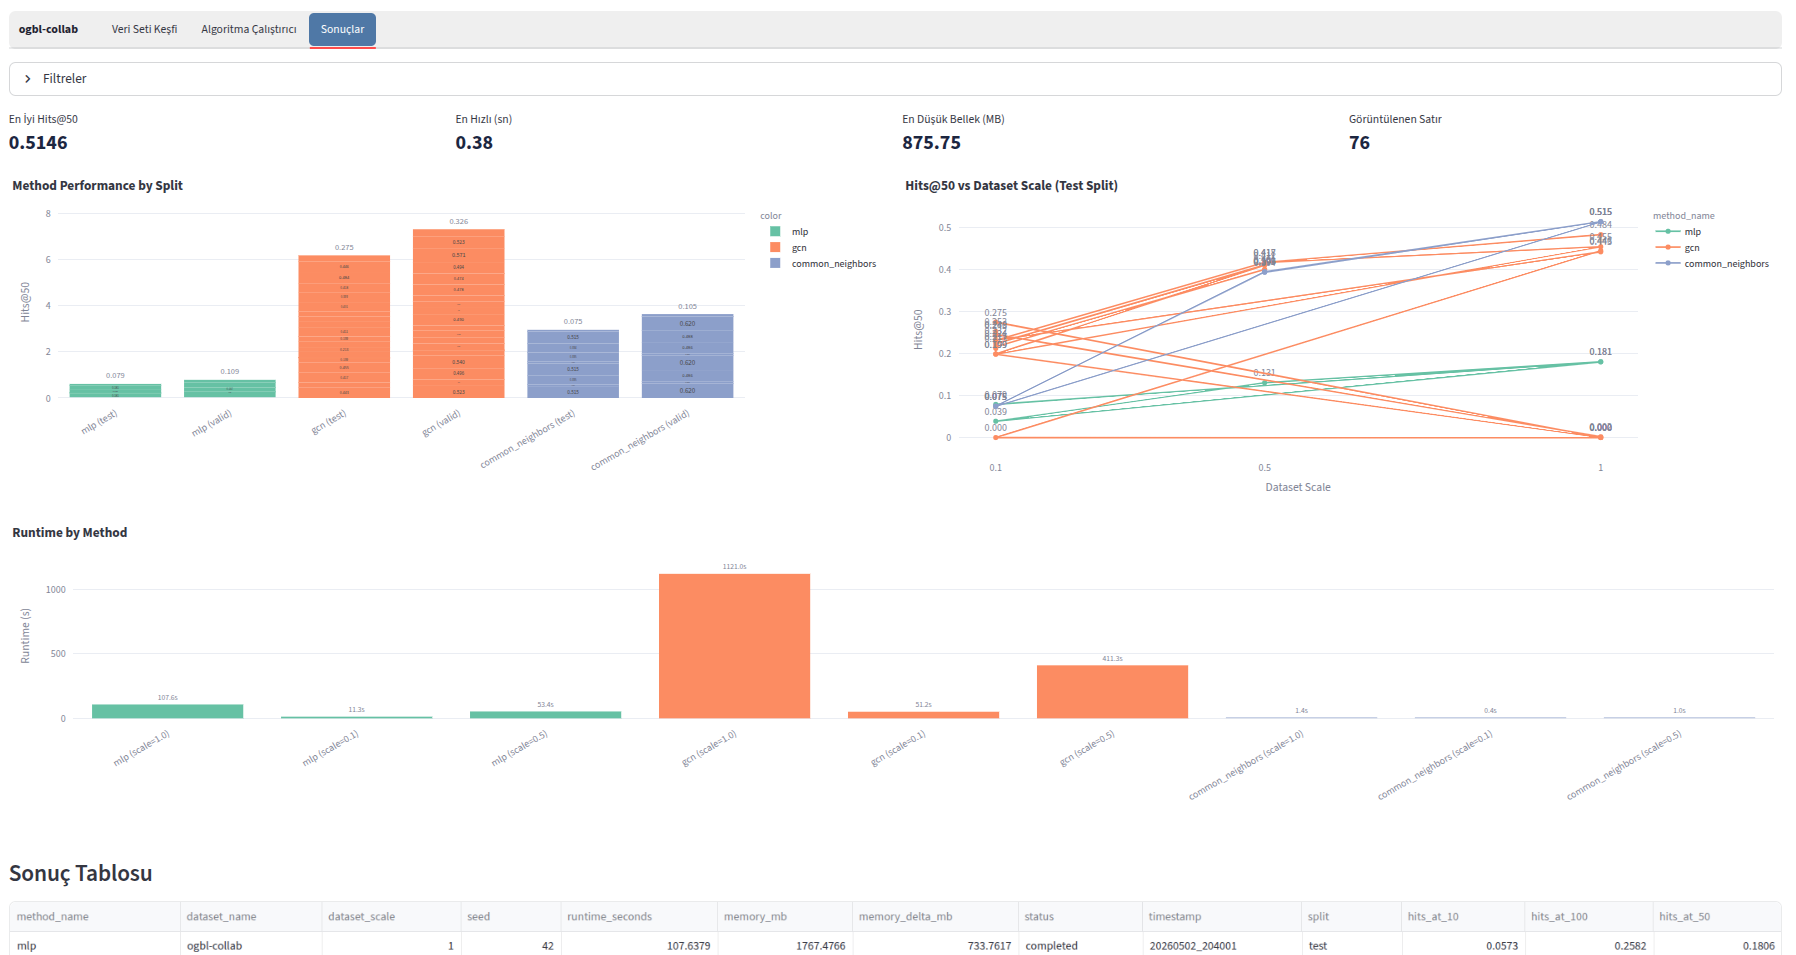
\includegraphics[width=0.85\textwidth]{figures/sonuclar.png}
\caption{Results Dashboard tab.}
\label{fig:screenshot_dashboard}
\end{figure}

\end{document}
